\section{Architecture}

The PADI-FS architecture is composed by three main components. First, the
metadata server which keeps the file's metadata and is replicated by three
replicas. Second, the data server which is responsible for storing the contents
of the files. Exists more than one data server, allowing the contents of
a given file to be replicated. And third, the client which is responsible for
making the requests.\\

The following figure is meant to illustrate the architecture of the system.\\

\begin{figure}[H]
	\center{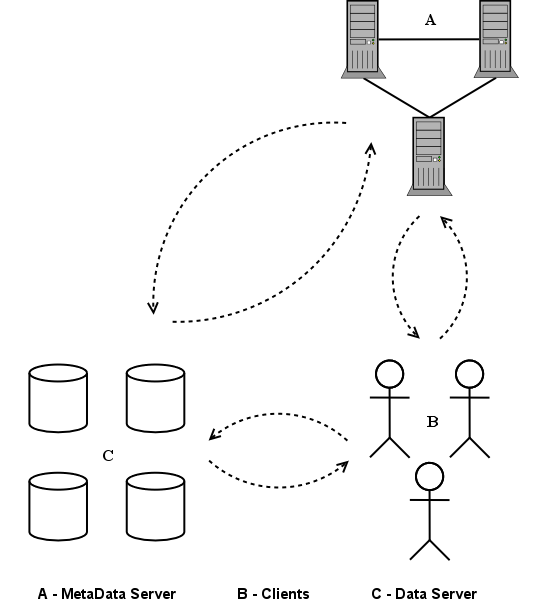
\includegraphics[width=0.4\textwidth]{PADIFS.png}}
  	\caption{System architecture.}
\end{figure}

These three components will be described in the sub-sections below to give
a deep insight on the way each component works and how their implementation
solves the different problems that can occur.

There is also a fourth component on the system, denominated Puppet Master,
which is a centralized controller that can issue commands to all the other
components. Because this component only exists to simplify testing and
debugging of the system, it's not described in this paper.

%------------------------------------------------------------------------- 
\subsection{Metadata Server}

Metadata servers maintain metadata information about the files stored
in the data servers. This metadata holds relevant information about
the files such as the file name, the number of servers used to store
the contents of the file, the minimum number of data server that should
be contacted during the read and write operations and a list of the
data servers that have the file stored. The metadata server also stores
information about the number of files each data server stores, which
servers are available or not and which files are open in clients.
The reason why we do this will be explained below on document.

As it was previously mentioned, there are 3 replicas of the metadata
server. The purpose of these replicas is to have the content of the
server replicated so that when a replica fails, there's another one
that can reply to the requests made. This replication is made in a
passive manner, which means that just one of the replicas will be
responsible for all the operations. The primary replica has to
synchronize its state with the secondary ones to make sure that all
the replicas store the same information at all time. Passive replication
is more useful in this system than active replication in a way that we
can tolerate two failures and have always a server to be able to reply to
any request made by the client.

\subsubsection{Handling Files}

The primary server can reply to several requests from the client. This
request are create, open, close and delete operations.
When a client send a request to create a file, the server saves a new
registry for that file with the information sent with the request. The
primary replica must inform the necessary data servers that they need to
create a local copy of the file and wait for them to reply back. Then
it increases the number of files for each server and sends the new 
entry to the other two replicas so they can be up to date. It's important 
to mention that when a data server is down, the metadata server will try 
to send the request to another server. If there are no more servers to 
send the request to, the metadata server will wait for the data server 
to come up to send it the information it needs to create the file. A 
secondary replica can also be down when the primary one sends its new 
information. When this happens, the primary server will not wait for 
the reply of the other server. Just after this exchange of requests and
replies, the metadata server tells the client it's all good and the file 
was successfully created.

When a client asks to delete a file, the metadata server decreases the
number of files for each server that holds the file and removes the 
corresponding entry from the table where all the information is stored. 
The system does not provide any functionality to clean the garbage that 
the data servers keep stored.

After creating a file, the client can open it. In this case, the metadata 
server sends the client all the information it has stored for that file.
The metadata server count how many clients are using each file, increases
this number when a client open and decreases when it close.
That way, the client is able to perform read and write operations. While 
the file is open, it cannot be copied if the data server that holds the 
file is not available.

The primary metadata, from time to time, pings the data servers to know 
which are available and which are not. When a data server is not 
available, the metadata server will try to migrate the files stored on 
that server to another one. The new server should be on the available list of
servers to avoid choosing the same. The copy of the files should happen only
if the file being copied isn't open. When the file is fully copied to other 
server, meaning the metadata already sent the request to it to create a 
new file and it did respond saying the file was created, the metadata 
server has to update the list of servers that hold that file. The downside 
of this process is that the file is no longer referenced to the 
old server but the file is still there and there's is not a proper way 
to remove it.

\subsubsection{Failure and Recovery of Metadata Servers}

All the replicas need to know if the primary replica is well and good to 
keep executing the requests that clients are making. To keep track of this, 
the primary server sends a heartbeat along with a log of the servers that 
are available and unavailable so they can update their own list. Supposing 
the primary replica is down and can't send the other replicas the heartbeat 
they're expecting, the replicas need to cover the primary so the client can 
keep asking for create, open or close operations. To do this, the replicas 
send each other their ID's and the one with the lower ID is the new primary
replica. If a replica does not receive any response from the other, it 
means that it is not available either and this replica has no choice but to 
be the new primary server. When a replica recovers, asks the others who is 
the primary server and updates its state accordingly. During all this process, 
metadata servers can't respond to any request from the clients.

%------------------------------------------------------------------------- 
\subsection{Data Server}

Data Servers store the content of one or more files. The content of each
file is stored using the local file system, in a local file with a
16-character ASCII string name generated by the Metadata Server. The
state and all files of the Data Server are written to disk.

Data Servers store files with a version composed by a
monotonically increasing number, that starts with 0, and a timestamp.
The files also have a byte array with the content of the file.

\subsubsection{Data Servers and Metadata Server}

The first action of a Data Server is to inform the Metadata Servers that
it is available to receive requests to store files from. The Metadata
Server should register the Data Server as available and reply to the Data
Server that the registration took success. The Data Server waits for the
reply and if it does not receive any, it resend the message. The secundary
Metadata Servers discard this message.

The Data Server sends a regular message, heart beat, to all the Metadata
Servers. The message is ignored by the two replicas, whether they are
available or not. This way, the Data Server does not have to keep
registered which Metadata Server is the primary and simplifies when
there was a change of primary Metadata Server, the Data Server does not
have to resend the message to the new primary.
This heart beat is useful to the primary Metadata Server keep track of
which servers are available to store new files and to avoid clients
from beeing waiting for Data Servers to come up to have a majority quorum.
We choose to not give the responsability to the Metadata Server of ask to
any Data Server if it is alive and wait for an answer because, in a large
system, the workload of the Data Servers will be lower compared to the
workload of the Metadata Servers. The exception is when multiple clients
are reading and writing intensively to the same few Data Servers. We
understood that this is an exception case. With this aproach, only one
message is sent from the Data Server to the Metadata Server trough the
network.

When the Data Server fails or freezes it stops sending heart beats to
the Metadata Servers. If the primary Metadata Server does not receive an
heart beat in a time window, it believes the Data Server is unavailable
and this servers stops receiving requests from de Metadata Server to
create new files.

Each time the Metadata Server asks the Data Server to create a new file
with a given name, the Data Server tries to create the new file and answers
to the Metadata Servers if the operation took success or not.

The Metadata Server may request one Data Server to send a copy of one file
to another Data Server. This request is treated as any other request.

\subsubsection{Reading and Writing to Data Servers}

Clients ask Data Servers to read or write files. This requests are
processed as they arrive to the server without having any priority neither
any reordering. It is simpler to buffer the requests as they arrive and to
perform them later.

Every file written in Data Servers have a version composed by a version
number that is incremented everytime the file is written and a timestamp
from the last writing. This timestamp let the Data Server to know if it is
receiving a version earlier than the version it stores.

When the Data Server is requested to store a new version of the file, it
checks if the new version is newer than the version that it stores, it
compares the timestamps and if it is earlier, it discards the version, else,
increments the version number of the file and stores it to disk.
This solution raises the problem of destroying the previous work of one
client when other, that read a previous file and edited it, asks the server
to write its version, overwriting the previous version, written by other
client, without updating its version with the content from the previous. To
avoid this, we could implement a solution similar to distributed revision
control systems, which would rise the complexity of the project.

%------------------------------------------------------------------------- 
\subsection{Client}

The client can create, open, read, write, close and delete files. When  it is created, it is provided the contact of the all metadata servers and which of these is primary server. 
The client can contact the primary metadata server to create, open, close or delete a file.

\subsubsection{Create} 

When client request to create a new file to the metadata servers, it specifies the name of the file, the number of data servers used to store the data and the number of data server that it needs to obtain a read and write quorum. The size of quorum can't exceed the number of data server used to store the file. 

\subsubsection{Open}

If client wants to open a file, it sends a request to primary metadata server to open a file, and obtains the information about the data servers where is stored the file content, the local name of these files in data servers and the size of read and write quorum.

\subsubsection{Read and Write}

In Reads and Writes, the client contacts directly data server, since it client already knows where is the file. During the write of the file in data servers, the client must block until receives the confirmation from the quorum of data servers. The size of this quorum is defined in metadada servers, when the file is created. Like in write, in read the client also block until the data server sends a response with read quorum.
If while the process request to read or write a file, the number of data servers that answer is less than required to obtain quorum, due to communication failures or if server can't answer, the client is put on hold and continues to try contact the data servers until get that quorum.
In the event of data server freeze, the messages that client sends are buffered. When it unfreezes, the server sends an answer for each request that is in the buffer. In this case, the client just consider the first answer, and it ignoring the other ones.
The client doesn't control the file version number. This number is controlled by data server.

\begin{itemize}
\item Default Read - The client makes a request to data server to read a file,  wait for majority quorum, and accept  that file even it is an older version.

\item Monotonic Read - The client makes a request to data server to read a file and waits for majority quorum to retrieve  a version equal or greater than.
\end{itemize}
